\documentclass{article}

\usepackage{graphicx}
\usepackage{fullpage}

\begin{document}

    \section{Introduction}
    
    When given a set of documents and a query we want to rank these documents in terms of relevance to the query.
    For example, given the query "cute kittens" we would expect that documents pertaining to kittens which are cute to be considered important and those pertaining to dogs to be ranked low.
    Traditional techniques for ranking involve hand crafted heuristcs or probabilitic approaches.

    A modern technique for ranking documents is called learning to rank.
    Learning to rank is a technique in which we use machine learning tools to rank documents when compared to a query.
    

    \section{Method}

    Our method is composed of two parts: (1) construct our ranking algorithm (2) evaluating new documents in relation to a query.

    \begin{itemize}
        \item Pre-process Data
        \item Create clusters
        \begin{itemize}
            \item Create cluster pairs
        \end{itemize}
        \item For each cluster, and cluster pairs, create a learner 
    \end{itemize}

    \begin{itemize}
        \item Given a set of documents for a query we create pairs of each document
        \item For each document pair we choose our learner based on which cluster 
        \item Using our pair rankings we construct a graph where those ranked higher have out edges to those ranked less
        \item From our graph we rank documents based on the number of out edges and in edges of a node.
        \begin{itemize}
            \item We use the ratio of out degrees to end degrees to select the current top ranking document
            \item once we have selected a document we remove it from the graph and repeat until there are no more documents
        \end{itemize}
    \end{itemize}

    \section{Results}

    \begin{figure}[th!]
        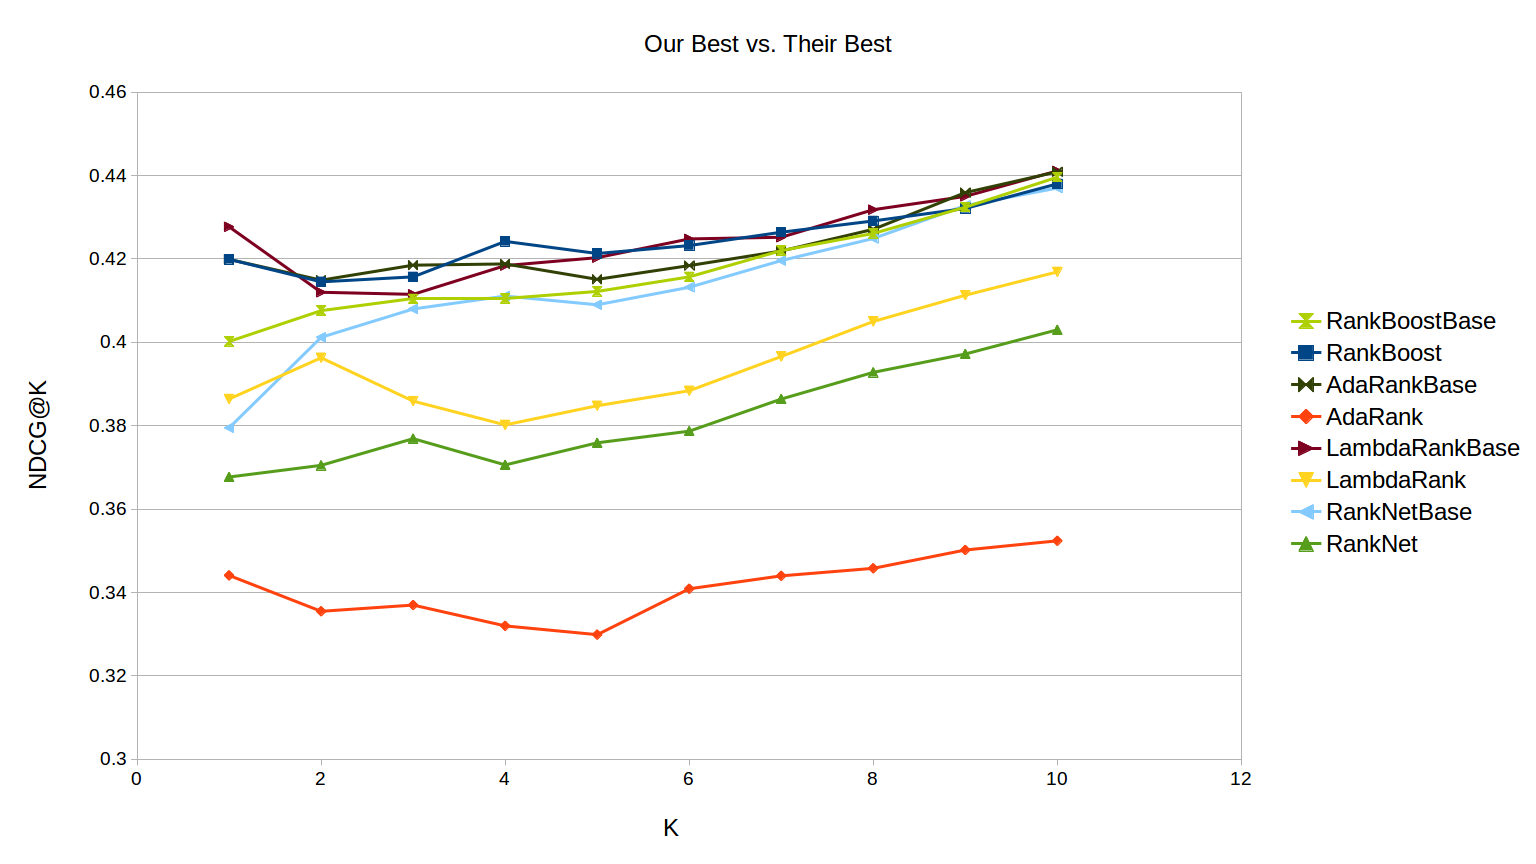
\includegraphics[keepaspectratio=true,scale=0.35]{images/best_of_each.png}
        \caption{Best of each base algorithm along with best results we can get using our method.}
        \label{fig:best_of_all}
    \end{figure}

    In figure~\ref{fig:best_of_all} we present each result for each underlying learner along with the best result using our method with each learn.
    For RankBoost and RankNet we acheve the best results with 5 clusters, for AdaRank and LambdaRank we acheive the best result with 2 clusters.
    RankBoost is the only underlying learner which results in better performance when we apply our method for K values of 2, 3, 4, 5, and 8.
    When using 8 clusters we only acheve better results when looking at the first document in the ranked list.     

    \subsection{RankBoost}
    
    When using RankBoost as our training algorithm our results see an improvement up to 2\%.  In figure~\ref{}  

    \begin{figure}[th!]
        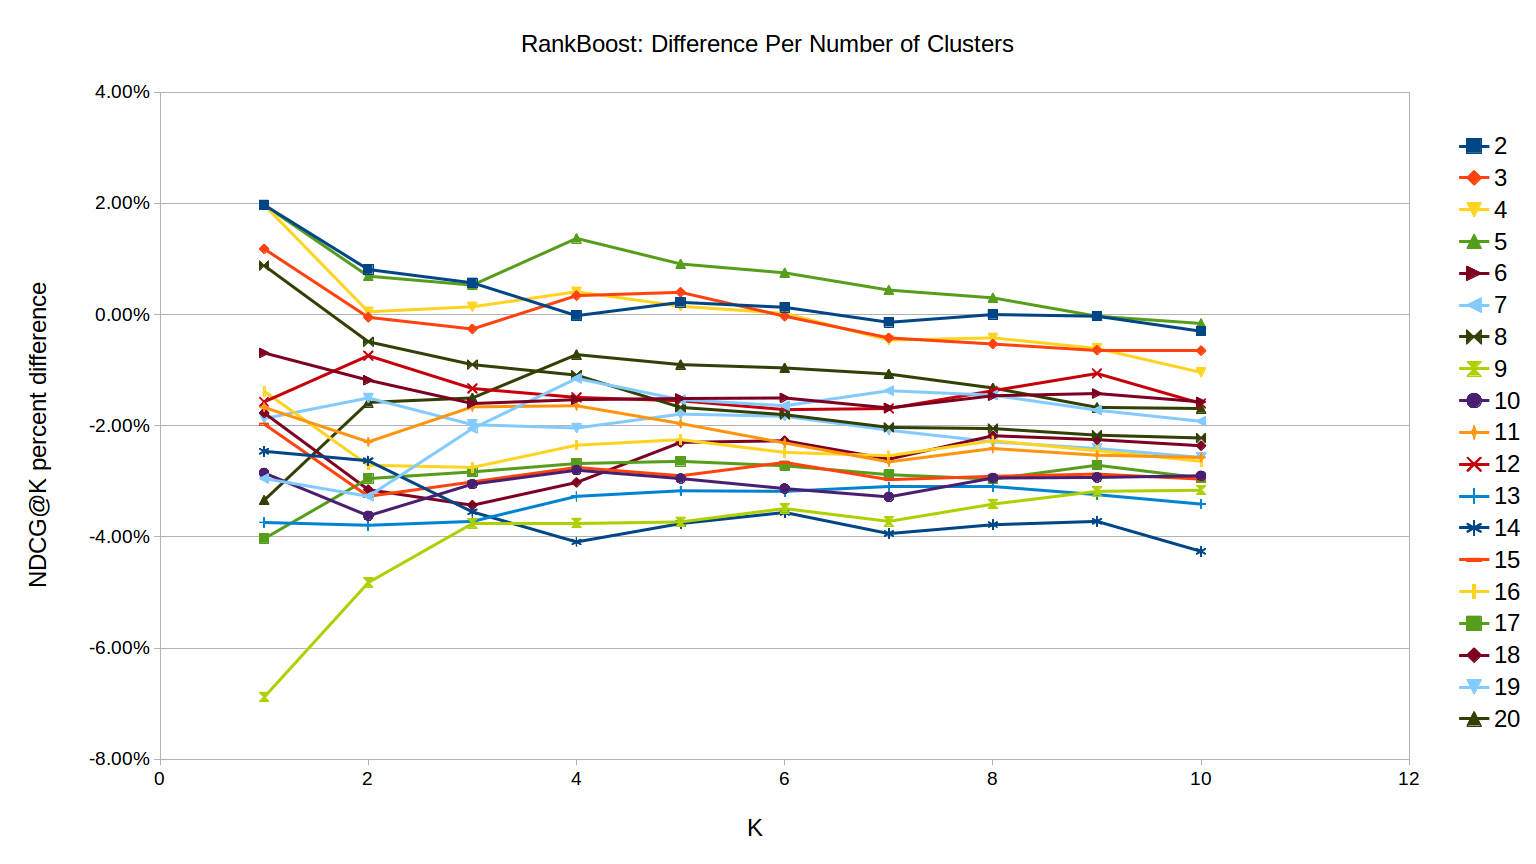
\includegraphics[keepaspectratio=true,scale=0.35]{images/rankboost_results.png}
    \end{figure}

    \subsection{AdaRank}

    \begin{figure}[th!]
        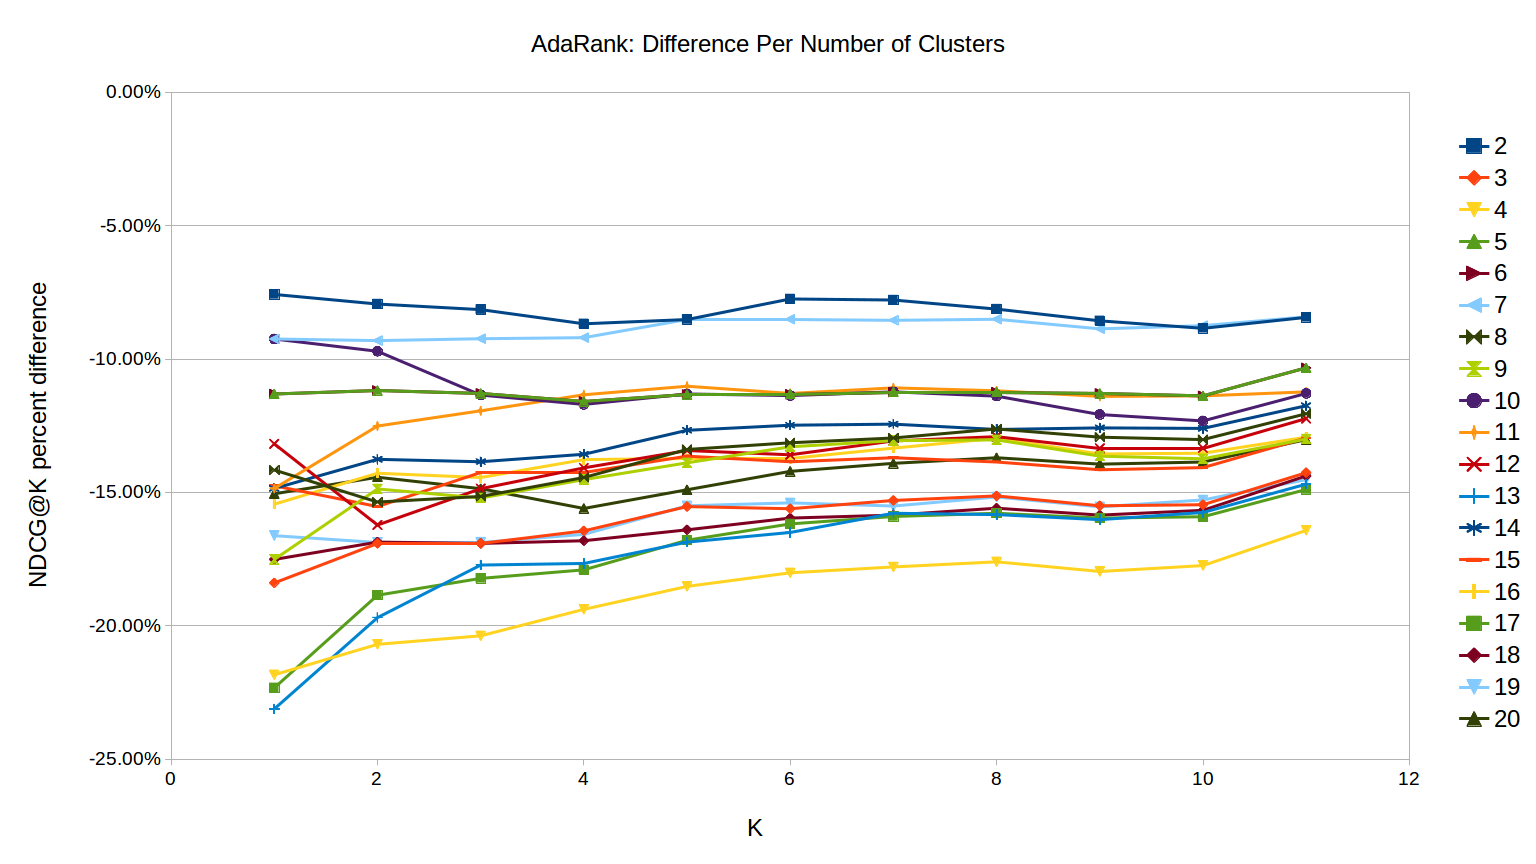
\includegraphics[keepaspectratio=true,scale=0.35]{images/adarank_results.png}
    \end{figure}

    \subsection{LambdaRank}

    \begin{figure}[th!]
        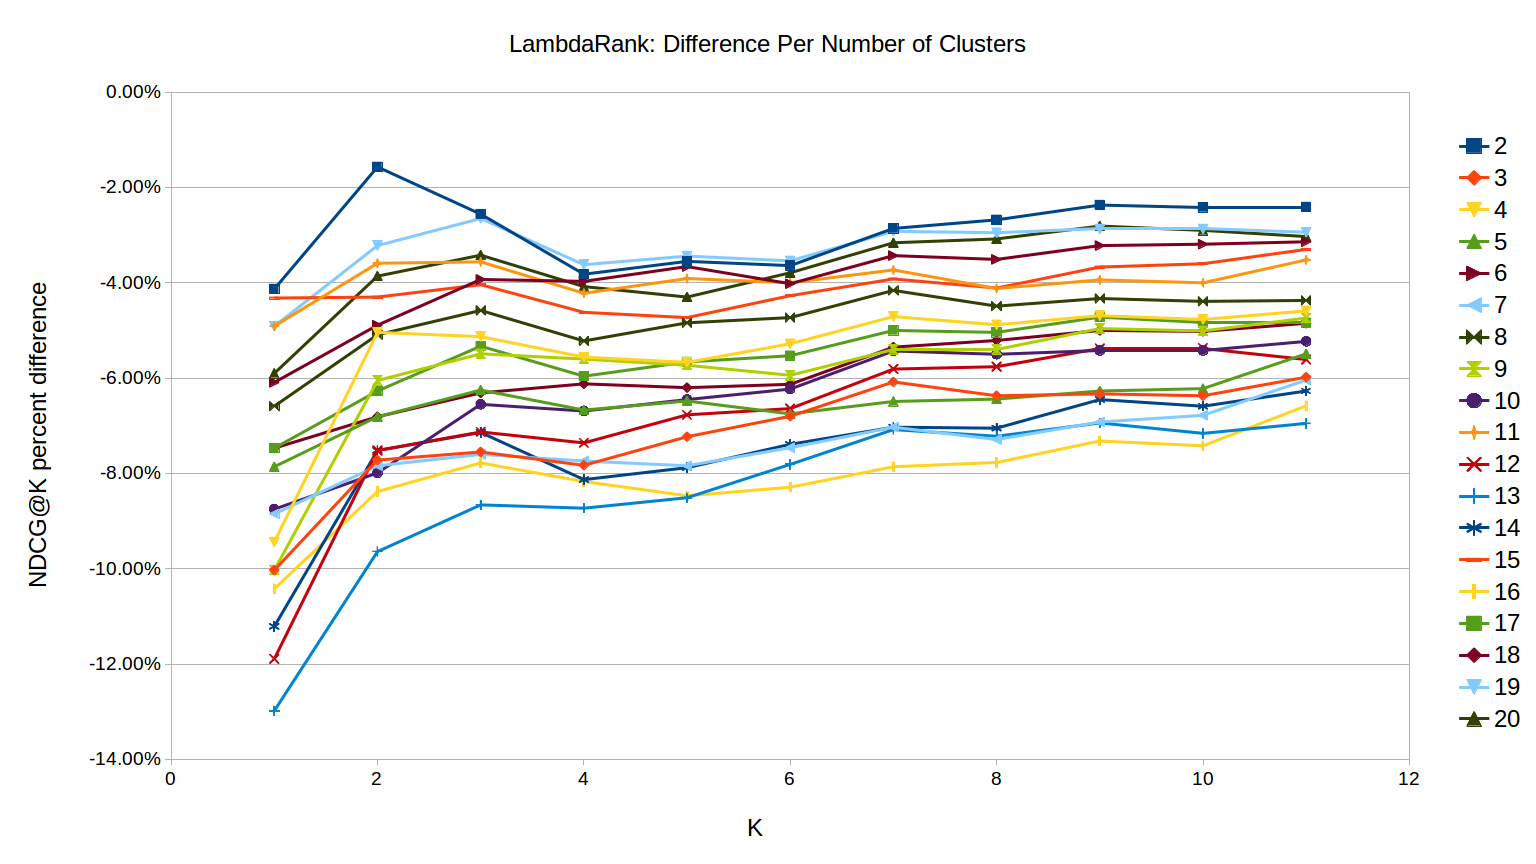
\includegraphics[keepaspectratio=true,scale=0.35]{images/lambdarank_results.png}
    \end{figure}


    \subsection{RankNet}

    \begin{figure}[th!]
        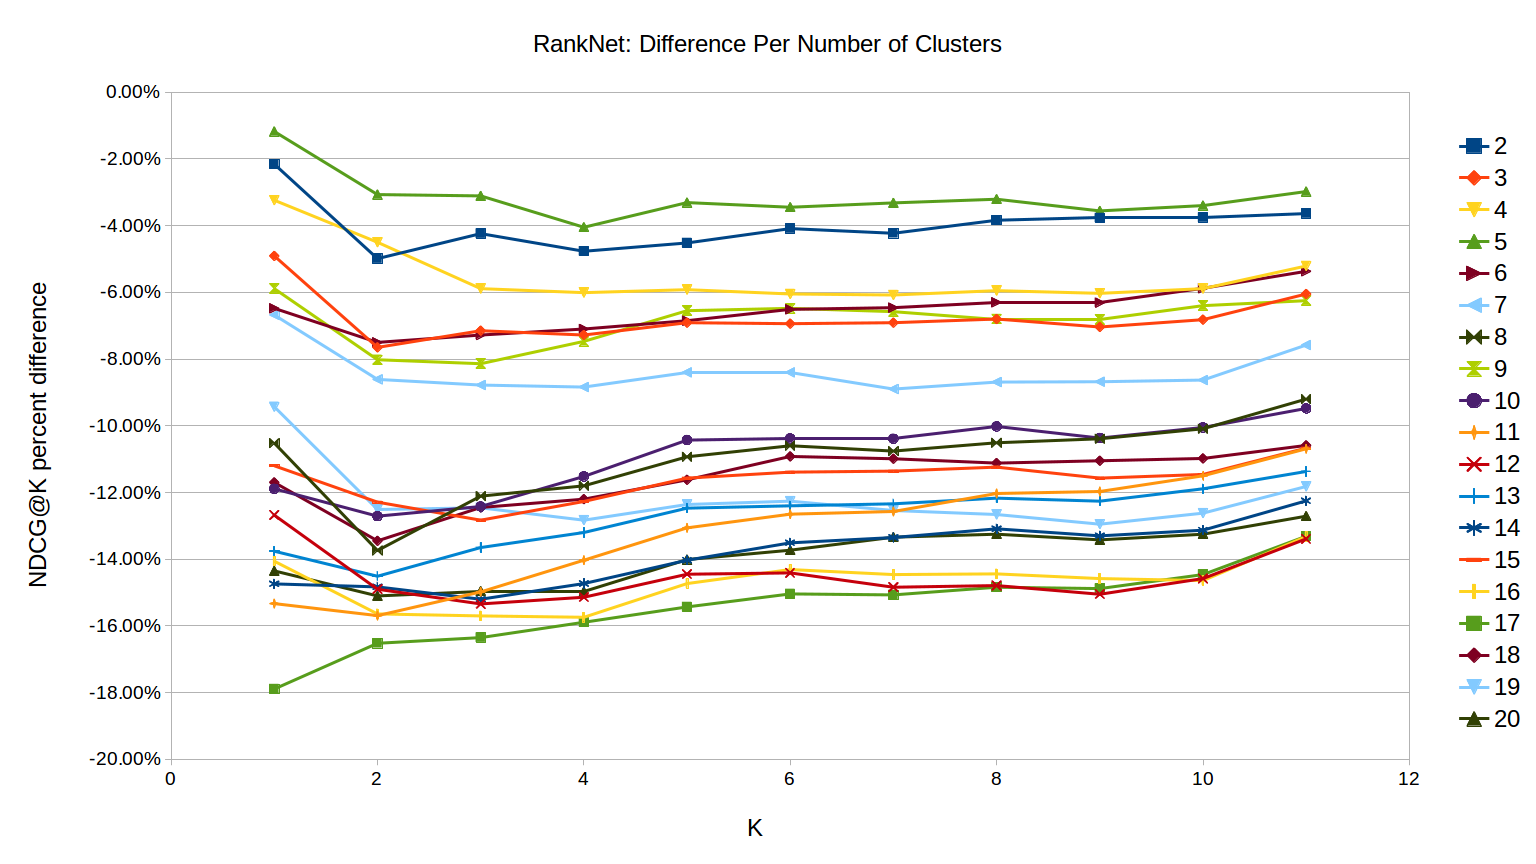
\includegraphics[keepaspectratio=true,scale=0.35]{images/ranknet_results.png}
    \end{figure}
  

\end{document}